\chapter{The acoustic space of voice quality in Santiago Laxopa Zapotec} \label{ch:acousticlandscape}

%--------------------------------------------------------------------------
\section{Introduction} \label{sec:acousticlandscape:intro}
%--------------------------------------------------------------------------

This chapter studies the acoustic dimension of voice quality in Santiago Laxopa Zapotec (SLZ) using a Multidimensional Scaling (MDS) analysis of acoustic data. MDS is a statistical method that reduces the dimensionality of a dataset and visualizes the relationships between data points. This study uses MDS to visualize the acoustic space of voice quality in SLZ. This analysis provides information on the acoustic correlates of voice quality in SLZ and contributes to our understanding of the phonetic properties of this underdocumented language.

This study is based on the work conducted by \citet{keatingCrosslanguageAcousticSpace2023} on the acoustic space of voice quality in 11 languages. However, this study focuses on a single language, SLZ, and provides a detailed analysis of the acoustic properties of voice quality in this language. The results of this study will contribute to our understanding of the phonetic properties of SLZ and how the acoustic properties of voice quality in this language compare with other languages.

%--------------------------------------------------------------------------
\section{Methods} \label{sec:acousticlandscape:methods}
%--------------------------------------------------------------------------
\subsection{Participants} \label{sec:acousticlandscape:participants}

This study uses data collected from 10 native speakers of SLZ during the summer of 2022. Participants were recruited from the community of Santiago Laxopa, Oaxaca, Mexico. All participants were native speakers of SLZ. The participants were between 18 and 60 years old and consisted of five males and five females.
\subsection{Recordings} \label{sec:acousticlandscape:recordings} 
The participants were asked to perform a word list elicitation task consisting of 72 words. These words were selected to elicit the entire range of types of voice quality in SLZ, including modal voice, the two kinds of creaky (i.e., checked and rearticulated), and breathy voice. The words were selected based on previous research conducted as part of the Zapotec Language Project at the University of California, Santa Cruz \citep{ZapotecLanguageProject}. 
Because participants were not literate in SLZ, the word list was prompted for them by asking them ``How do you say [word in Spanish]?" by myself and another researcher in Zapotec. Participants were asked to respond with the desired word in the carrier phrase \textit{Shnia' [WORD] chonhe lhas} ``I say [WORD] three times.'' which was repeated three times. These utterances were recorded in a quiet environment using a Zoom H4n digital recorder. The recordings were saved as 16-bit WAV files with a sampling rate of 44.1 kHz.

\subsection{Acoustic measuring} \label{sec:acousticlandscape:analysis}
These resulting audio files were then processed in Praat to isolate the vowel portion of each word. The onset of the vowel was set to the second glottal pulse after the onset, and the offset of the vowel was set to the last glottal pulse before the decrease in amplitude at the end of the vowel \citep{garellekAcousticDiscriminabilityComplex2020}. The vowel was then extracted and saved as a separate file for analysis.

These vowels were fed into VoiceSauce \citep{shueVoiceSauceProgramVoice2011} to generate the acoustic measures for the studies discussed in this dissertation. Because many acoustic measures are based on the fundamental frequency, this measure was calculated using the STRAIGHT algorithm from \citep{kawaharaInstantaneousfrequencybasedPitchExtraction1998}. The STRAIGHT algorithm estimates the fundamental frequency in millisecond (ms) intervals. Once the fundamental frequency is calculated, VoiceSauce then uses an optimization function to locate the harmonics of the spectrum, finding their amplitudes.

VoiceSauce then uses the Snack Sound toolkit \citep{sjolanderSnackSoundToolkit2004} to find the frequencies and bandwidths of the first four formants, also at millisecond intervals. The amplitudes of the harmonics closest to these formant frequencies are located and treated as the amplitudes of the formants. These formant frequencies and bandwidths are used to correct the harmonic amplitudes for the filtering effects of the vocal tract, using \citeauthor{iseliAgeSexVowel2007}'s \citeyear{iseliAgeSexVowel2007} extension of the method employed by \citet{hansonGlottalCharacteristicsFemale1997}. Each vowel was measured across ten equal time intervals, resulting in 22890 data points in total. These measures were then z-scored by speaker to reduce the variation between speakers and provide a way to compare the different measures directly on the same scale.

\subsection{Data processing} \label{sec:acousticlandscape:processing}
Data points with an absolute z-score value greater than three were considered outliers and excluded from the analyses in the dissertation. The Mahalanobis distance was calculated in the F1-F2 panel within each vowel category. Each data point with a Mahalanobis distance greater than six was considered an outlier and excluded from the analysis.  

Energy was excluded if it had a zero value and then log-transformed to normalize its right-skewed distribution. Afterward, the resulting log-transformed data was z-scored, and any data point with a z-score greater than three was excluded. This outlier removal resulted in 1918 data points being removed. 

After removing the outliers, I calculated residual H1* for the remaining data points following \citet{chaiH1H2Acoustic2022}. First, a linear mixed effects model was generated with the z-scored H1* as the response variable and the z-scored energy as the fixed effect. The uncorrelated interaction of the z-scored energy by speaker was treated as random. The energy factor resulting from this linear mixed-effects model was extracted. Finally, the z-scored H1* was the product of the z-scored energy and the energy factor subtracted from it.

Once these steps were completed, the mean of each vowel and speaker of the fifth and sixth intervals was taken. This is similar to what \citet{keatingCrosslanguageAcousticSpace2023} did by taking the middle of the vowel for their analysis. This choice minimizes the effect of the onset and offset of the vowel on the acoustic measures, which are more likely to be affected by the surrounding consonants and should give us the most accurate representation of the vowel quality. Because z-scores were used, this resulted in negative measures, which presents a problem for MDS analyses. To correct for this, I added the absolute value of the minimum z-score to each measure. This results in a dataset that still preserves the relative differences in the scores while providing a dataset that is all positive for the MDS analysis.

\subsection{Statistical analysis} \label{sec:acousticlandscape:statistics}

Using a multidimensional scaling (MDS) analysis is a statistical method of reducing the dimensionality of a dataset to visualize the relationships between the data points \citep{kruskalMultidimensionalScaling1978}. This is especially true when many variables could contribute to the data. In the case of voice quality, this is especially true. As shown in \citet{kreimanUnifiedTheoryVoice2014,kreimanValidatingPsychoacousticModel2021,garellekAcousticDiscriminabilityComplex2020}, voice quality is psychoacoustically complex and a single measure is not enough to capture the full range of voice quality. Instead, multiple measures are required that function as cues for the different types of voice quality. For example, a vowel characterized as having a breathy voice has an elevated spectral-slope and a lower harmonics-to-noise ratio than modal voice. A creaky voice has a lowered spectral-slope and a lowered harmonics-to-noise ratio. 

Because MDS analyses that contain many variables can result in rather unmeaningful results, I chose to focus on the speaker x voice quality interaction. This allows us to see how speakers differ in their production of the different voice qualities. This choice to focus on speaker x voice quality means that each speaker's production of each of the four phonation contrasts is represented as a single point in the MDS plot (e.g., one point for speaker 1's modal voice, one for speaker one's checked voice, one for speaker one's rearticulated voice, and one for speaker one's breathy voice). This is similar to what \citet{keatingCrosslanguageAcousticSpace2023} did in their study of the acoustic space of voice quality in 11 languages, except that they compared the language x voice quality interaction. Both of these interactions show us similar information. One shows us within a language, while the other shows us between languages.

The MDS analysis was conducted in R using the  `metaMDS' function in the `vegan' package. The Manhattan distance was used to estimate the physical differences between the speaker x voice quality pairs. Because the distances are non-Euclidean, the MDS analysis was conducted using the non-metric option. 

This algorithm resulted in a solution that involves several different dimensions. The number of dimensions retained directly affects how well the original data is captured. Too many dimensions and the data are overfitted; too few, and the data are underfitted. To determine the number of dimensions to retain, I used a scree plot to plot the stress of each dimension. The elbow of the curve was identified as the correct number of dimensions for analysis. Figure~\ref{fig:stress_plot} shows that most data is captured in a two-dimensional space. The third dimension adds more subtle information about the voice quality.

\begin{figure}[!h]
    \centering
    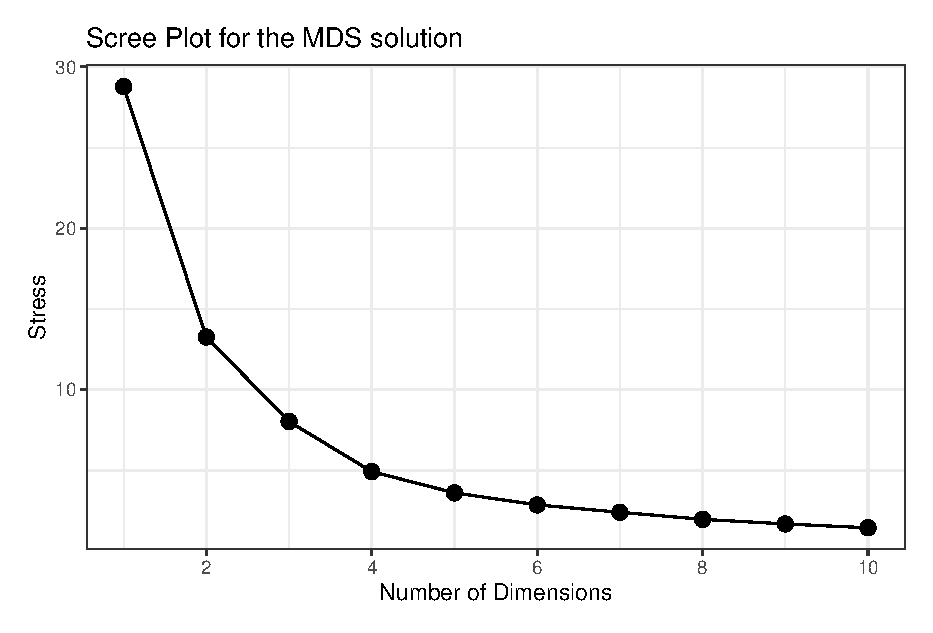
\includegraphics[width = 0.9\linewidth]{images/stress_plot.eps}
    \caption{Scree plot for the MDS analysis.}
    \label{fig:stress_plot}
\end{figure}
%--------------------------------------------------------------------------
\section{Results} \label{sec:acousticlandscape:results}
%--------------------------------------------------------------------------
\subsection{Acoustic space of voice quality} \label{sec:acousticlandscape:space}
As mentioned above, the results of the MDS analysis can be represented in a two-dimensional space, as shown in Figure~\ref{fig:nmds12}. In this and all subsequent plots, the breathy voice is represented by black, checked voice with orange, rearticulated voice with green, and modal voice with blue. Overall, we see that the breathy voice is located to the left of the plot, checked and rearticulated voices are tending to the right, and the modal voice is located in the center along the first dimension. The second dimension shows a modal and nonmodal split, with modal voice at the bottom of the plot and nonmodal voice at the top.
\begin{figure}[!h]
    \centering
    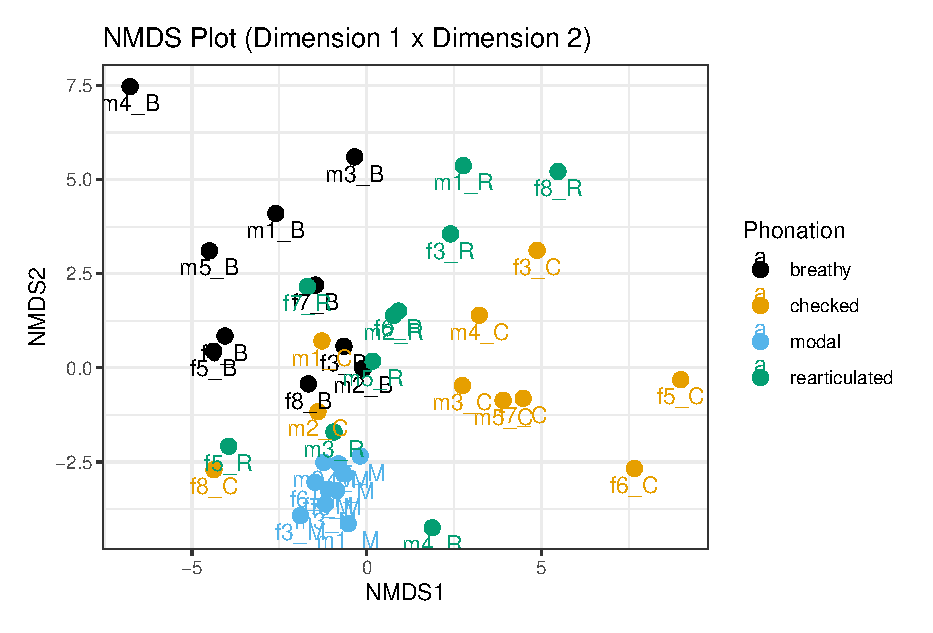
\includegraphics[width = 0.9\linewidth]{images/nmds12.eps}
    \caption{Two-dimensional MDS solution showing the first and second dimensions.}
    \label{fig:nmds12}
\end{figure}
    
As mentioned above, the third dimension adds more information about voice quality. Adding the third dimension helps spread the groups along the first dimension, as shown in Figure~\ref{fig:nmds13}. We see that breathy vowels are located at the top of the plot, and the two types of creaky voices (checked and rearticulated) are at the bottom. 

\begin{figure}[!h]
        \centering
        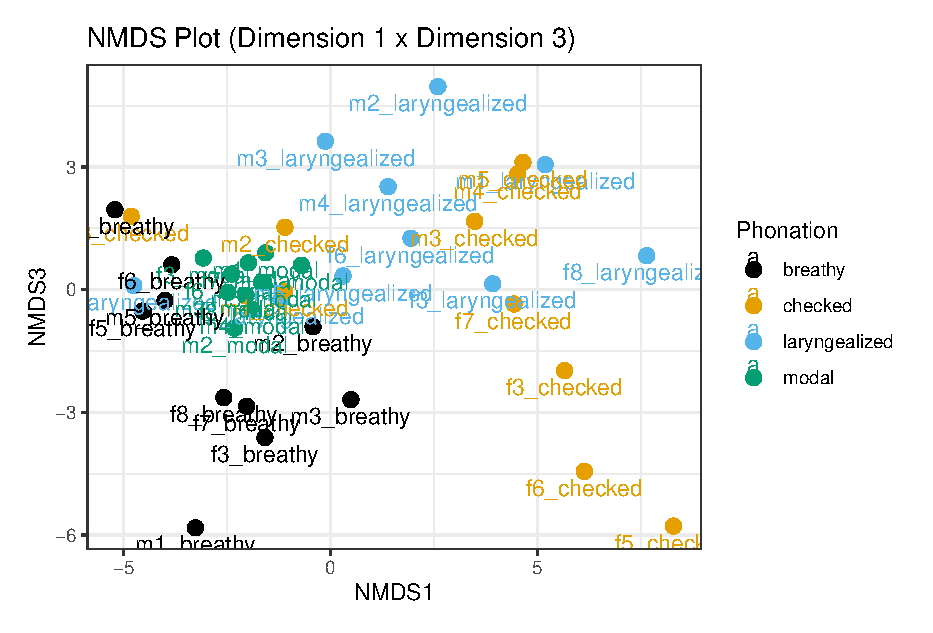
\includegraphics[width = 0.9\linewidth]{images/nmds13.eps}
        \caption{Two-dimensional MDS solution showing the first and third dimensions.}
        \label{fig:nmds13}
\end{figure}
    
When adding the third dimension to the second, we see that the breathy voices become separated from the other nonmodal voice qualities, as shown in Figure~\ref{fig:nmds23}. 

\begin{figure}[!h]
    \centering
    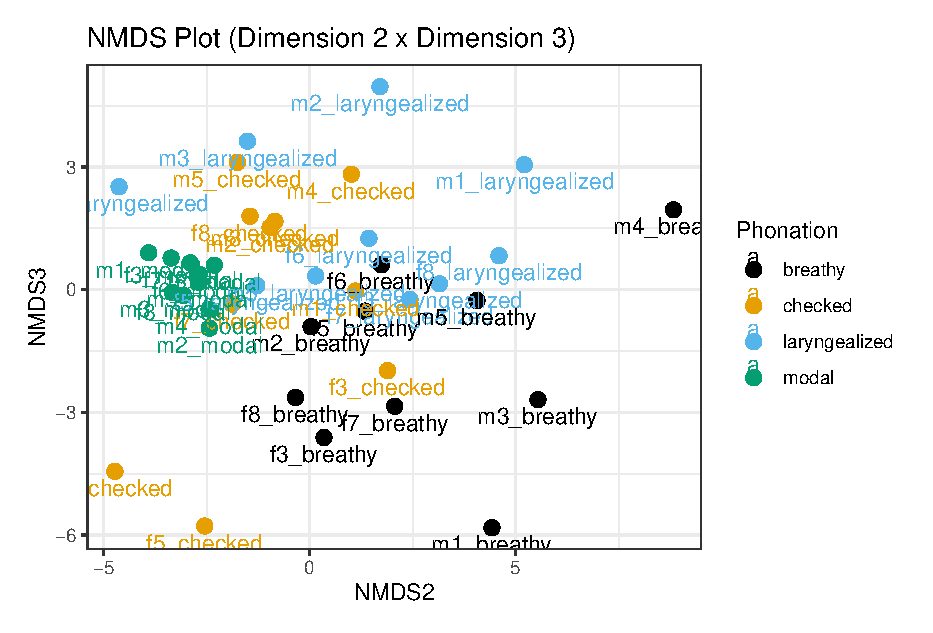
\includegraphics[width = \linewidth]{images/nmds23.eps}
    \caption{Two-dimensional MDS solution showing the second and third dimensions.}
    \label{fig:nmds23}
\end{figure}


\subsection{Acoustic correlates of voice quality} \label{sec:acousticlandscape:correlates}

An additional step to MDS analysis involves testing which acoustic measures contribute the most weight to the different dimensions. Table~\ref{tab:acoustic_correlates} shows the results of this test. In each of the three dimensions of the MDS analysis, the acoustic measures with the highest weight are shown in bold. In the case of the first and second dimensions (D1 and D2), the acoustic measures that have weights higher than those of other parameters are in boldface (weights > 4.0). In the case of the third dimension (D3), the acoustic measures that have weights higher than those of other parameters are in boldface (weights > 3.0). 

We see that for D1, the acoustic measures that have the highest weight on the first dimension are the amplitudes for the first three formants (i.e., A1*, A2*, A3*) and HNR < 500 Hz (i.e., a harmonics-to-noise ratio for everything from 0 to 500 Hz). For D2, the acoustic measures with the highest weight are H1*-A1*, H1*-A2* (i.e., spectral-slope measures), and the amplitudes of the first two formants. For D3, we see that HNR < 1500 HZ, HNR < 2500 Hz, HNR < 3500 Hz, and Residual H1* and H2* have the highest weights.

\begin{table}[ht]
    \centering
    \caption{Weight of each acoustic measure along each of the three dimensions indicated by the MDS solution (D1, D2, D3). Parameters that have weights higher than other parameters are in bold (weights > 4.0 for D1 and D2, and weights > 3.0 for D3).} 
    \label{tab:acoustic_correlates}
    \begin{tabular}{lrrr}
    \hline
    Acoustic Measure & D1 & D2 & D3 \\ 
    \hline
    H1*-H2* & 1.03 & 1.01 & 0.39 \\ 
    H2*-H4 & 1.15 & 3.98 & 2.13 \\ 
    H1*-A1* & 2.22 & \textbf{5.15} & 1.84 \\ 
    H1*-A2* & 2.93 & \textbf{4.66} & 1.00 \\ 
    H1*-A3* & 2.37 & 3.24 & 0.90 \\ 
    H4*-H2k* & 1.47 & 0.31 & 1.59 \\ 
    H2k*-H5k* & 3.73 & 0.73 & 0.84 \\ 
    residual H1* & 1.75 & 0.97 & \textbf{4.24} \\ 
    H2* & 1.76 & 0.94 & \textbf{4.09} \\ 
    H4* & 0.79 & \textbf{4.28} & 0.10 \\ 
    A1* & \textbf{4.96} & \textbf{5.48} & 0.17 \\ 
    A2* & \textbf{5.30} & \textbf{4.90} & 1.38 \\ 
    A3* & \textbf{4.54} & 2.91 & 1.11 \\ 
    CPP & \textbf{4.08} & 0.10 & 1.68 \\ 
    HNR < 500 Hz & \textbf{5.66} & 1.47 & 1.81 \\ 
    HNR < 1500 Hz & 3.95 & 2.68 & \textbf{3.08} \\ 
    HNR < 2500 Hz & 3.15 & 1.63 & \textbf{3.42} \\ 
    HNR < 3500 Hz & 2.86 & 0.55 & \textbf{3.19} \\ 
    Strength of Excitation & 2.09 & 0.78 & 0.36 \\ 
    SHR & 2.39 & 0.50 & 0.47 \\ 
    Energy & 2.22 & 3.91 & 0.64 \\ 
    \hline
    \end{tabular}
\end{table}

%--------------------------------------------------------------------------
\section{Discussion} \label{sec:acousticlandscape:discussion}
%--------------------------------------------------------------------------

The results of the MDS analysis show that the acoustic space in which SLZ's voice quality occupies is similar to other languages. Similar to what \citet{keatingCrosslanguageAcousticSpace2023} found in their study, the first dimension appears to roughly be similar to the open quotient of the glottis as proposed by \citet{gordonPhonationTypesCrosslinguistic2001}. In this model, voice quality is seen as the result of the glottis being more open or closed during phonation. The more open the glottis, the more breathy the phonation will be. The more closed the glottis, the more creaky the phonation will be. This model from \citet{gordonPhonationTypesCrosslinguistic2001} is shown in Figure~\ref{fig:phonation_types}.

\begin{figure}[h!]
    \centering
    \begin{tikzpicture}
        % Draw the line with arrows at both ends
        \draw[<->, line width=0.5mm] (0,0) -- (10,0);
        
        % Labels underneath the line
        \node[below] at (0,0) {[h]};
        \node[below] at (2,0) {Breathy};
        \node[below] at (5,0) {Modal};
        \node[below] at (8,0) {Creaky};
        \node[below] at (10,0) {[ʔ]};
        
        % Labels above the line
        \node[above] at (0,0) {Open Glottis};
        \node[above] at (10,0) {Closed Glottis};
    \end{tikzpicture}
    \caption{A diagram showing the relationship between breathy, modal, and creaky phonation types. Based on \citet{gordonPhonationTypesCrosslinguistic2001}.}
    \label{fig:phonation_types}
\end{figure}

As mentioned above, the measures that contribute the most to this first dimension are the amplitudes of the first three formants, CPP, and Harmonics-to-Noise Ratio < 500 Hz. Interestingly, even though this dimension is similar to the open-quotient model put forward by \citet{gordonPhonationTypesCrosslinguistic2001}, we do not observe measures traditionally associated with the open-quotient (i.e., spectral-slope). Instead of seeing traditional spectral-slope measures, we find the three formant amplitudes used to normalize the amplitude of the fundamental like in the measures H1*-A1*, H1*-A2*, and H1*-A3*. This suggests that the first dimension is more about the formants' amplitude than the signal's spectral-slope. This is combined with CPP and HNR < 500 Hz, which measures the harmonics-to-noise ratio for the first 500 Hz of the signal. This suggests that the first dimension is also concerned with the amount of noise in the signal.

The second dimension divides the space into modal versus nonmodal voice quality. The acoustic measures that contribute the most weight to this dimension are the spectral-slope measures H1*-A1* and H1*-A2* and the harmonic amplitudes of H4*, A1*, and A2*. This suggests that the second dimension is more about the spectral-slope of the signal than about the amount of noise in the signal. This is interesting given that traditional spectral-slope measures are associated with the open-quotient model of voice quality \citep{holmbergComparisonsAerodynamicElectroglottographic1995,kreimanMeasuresGlottalSource2007,garellekModelingVoiceSource2016,garellekPhoneticsVoice2019,chaiH1H2Acoustic2022}.

The third dimension adds more information on nonmodal voice quality. Figure~\ref{fig:nmds13} and Figure~\ref{fig:nmds23}, this third dimension separates the breathy voice from the other nonmodal phonation types. The measures contributing the most to this dimension are the harmonics-to-noise ratio for the first 1500 Hz, 2500 Hz, and 3500 Hz. In addition, the residual H1* and H2* have the highest weights, which is interesting given that residual H1* has been argued to be a more robust measure of the spectral-slope of the signal than traditional spectral-slope measures \citep{chaiH1H2Acoustic2022,brinkerhoffResidualH1Measure2024}. Furthermore, as discussed in Chapter~\ref{ch:residual_h1}, residual H1* represents the voice quality in SLZ better than H1*-H2* and H1*-A3*. This dimension is characterized by the harmonics-to-noise ratios for the first 1500 Hz, 2500 Hz, and 3500 Hz. This suggests that the third dimension is more about the signal's spectral quality than about the formants' amplitude. This is combined with residual H1* and H2*, which are measures of the spectral-slope of the signal.

%--------------------------------------------------------------------------
\section{Conclusion} \label{sec:acousticlandscape:conclusion}
%--------------------------------------------------------------------------

Although the discussion has predominately been about the weights of the measures that contribute to the different dimensions, it is important to note that the measures are not independent of each other. Instead, all of the measures contribute to the acoustic space of voice quality in SLZ to some extent or another. Just because a measure has a low weight does not mean that it does not contribute to the acoustic space, but it is still important to understand the acoustic space in SLZ. Rather than thinking of the measures as independent of each other, it is better to think of them as a group of measures that work together to create the acoustic space of voice quality in SLZ. This is especially true given the fact that the MDS analysis is a reduction of the data to a few dimensions. This analysis offers a snapshot of the voice quality acoustic space in SLZ, but is not the full picture. 

Additionally, as will be discussed in Chapter~\ref{ch:bagging}, another way in which we can determine which measures are the most important is by performing a bootstrap aggregating version of a classification and regression tree analysis \citep{breimanClassificationRegressionTrees1986,breimanBaggingPredictors1996}.